\section[MEX 1-1: Swelling of red salt clay]{Model-Experiment-Exercise MEX 1-1:\\Swelling of red salt clay}
\label{sec:mex05}
%------------------------------------------------------------------------------
\Authors{Amir Shoarian Sattari, Keita Yoshioka, Mathias Nest, Christopher R\"olke}
%------------------------------------------------------------------------------
This exercise (MEX 1-1) investigates the closure or opening of the micro pathways by swelling process in red salt clay. Both numerical and experimental approaches are implemented to understand the governing factors, which result in materials behavior change during the swelling process. The experimental setup is described in section \ref{sec:t4swell}.
\index{swelling processes}

\subsection{Experiment}

\begin{figure}[ht]
\centering
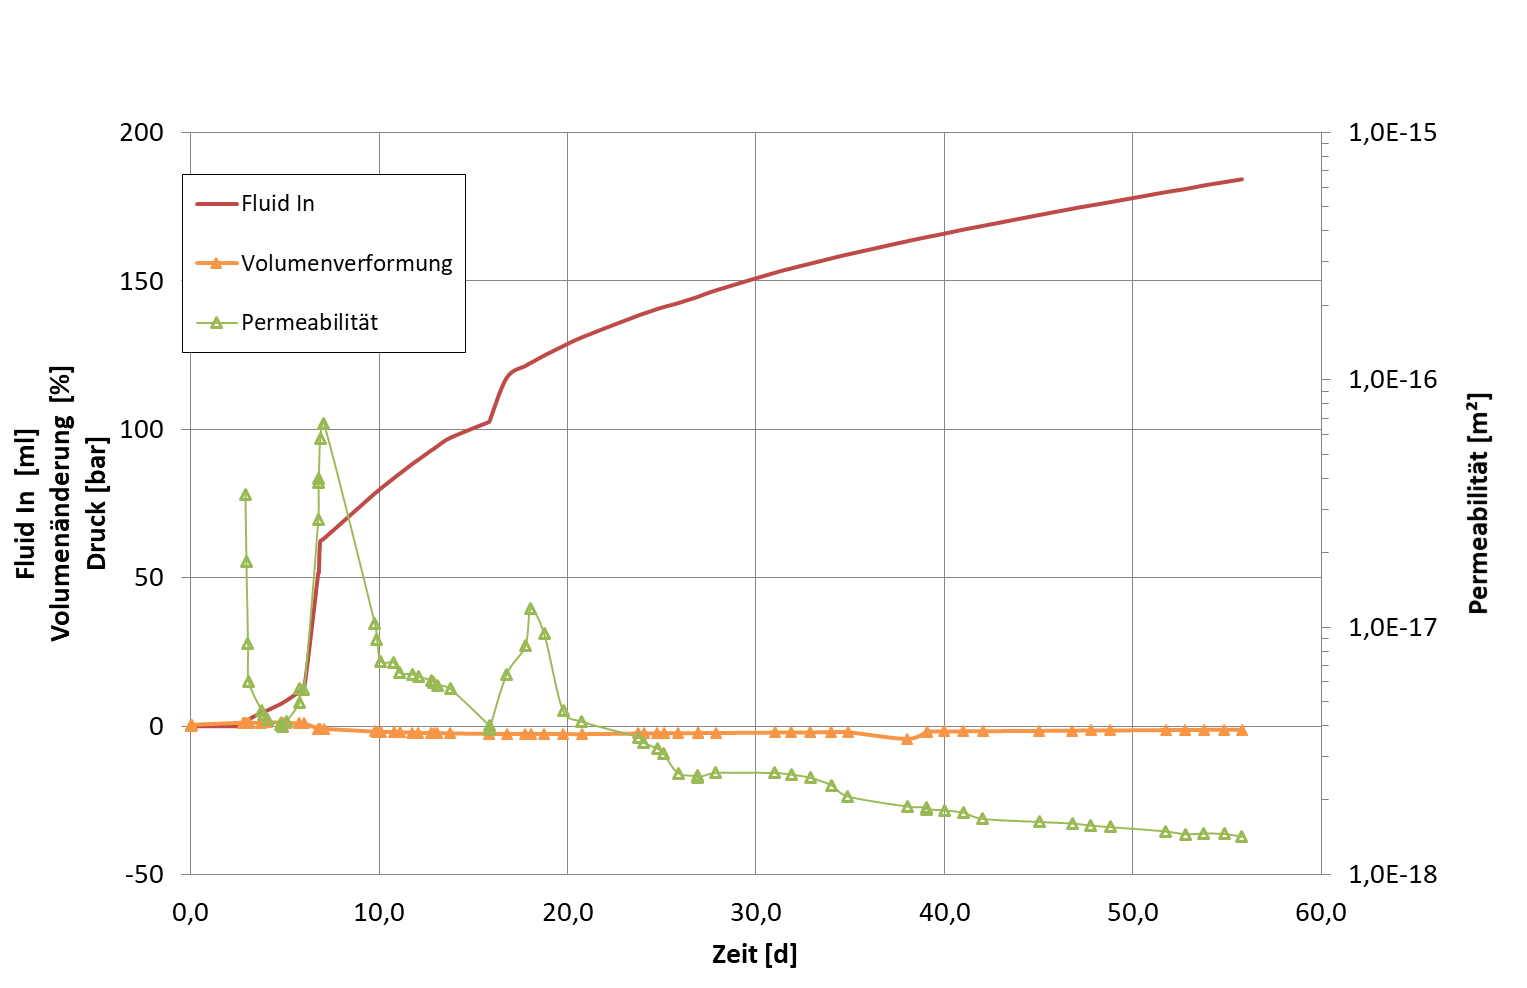
\includegraphics[width=0.8\textwidth]{figures/IfG-T4-results.png}
\caption{Results of the 8 week swelling test of T4 clay.}
\label{fig:t4swellresults}
\end{figure}

The experiment was conducted on a sample of dry red salt clay from the Aller series (T4) of the Zechstein in northern Germany. The experiment ran for 8 weeks, under isostatic stress conditions of 4 bar, and a brine pressure of 1 bar. 

Figure \ref{fig:t4swellresults} shows the amount of fluid that went into the sample (red), the change of the volume of the medium which applies the surrounding pressure (orange), and the permeability (green). We see that during the first three weeks the brine modifies the clay, and pathways are opened and closed. Apart from the wetting of the clay this may also be due to some salt going into solution and recrystallization. After this the permeability behaves more smoothly, and decreases with time. At all times the volume of the surrounding medium was below its initial value, indicating that swelling took place. 

%------------------------------------------------------------------------------
\subsection{Model approach}
\subsubsection*{Lattice element model}

With the application of the lattice model, the simulation of the swelling process in red salt clay sample is investigated. The experimental data provided by IfG Leipzig are used to determine the initial permeability and hydraulic aperture values. The effect of anisotropy is not investigated both in experimental and numerical approaches. The initial permeability value is assumed to be equal to $k_{per}=1\times10^{-16} [m^2]$. The initial hydraulic conductivity ($k_{h}$) is calculates based on,

\begin{align}
\label{eq:LEM_ME5_1}
\begin{split}
k_{h}=\frac{k_{per}\rho_fg}{\nu_f}
\end{split}
\end{align}

where $\nu_f=8.9\times{10}{^{-4} [Pa.s]}$, $\rho_f=998 [\frac{kg}{m^3}]$ and $g=9.8 \frac{m}{s^2}$. The $k_{h}$ is equal to $1.1x10^{-9} [m.s^{-1}]$. The initial hydraulic aperture or length of the interface element is calculated as,

\begin{align}
\label{eq:LEM_ME5_2}
\begin{split}
a_h=\sqrt{\frac{12k_h\nu_f^{k}}{g}}=3.67\times10^{-8}
\end{split}
\end{align}

where $\nu_f^{k}=1.004\times{10}{^{-6} [m^2.s^-1]}$. The calculated parameters then are transformed into lattice model to simulate the swelling and change of the permeability with swelling process. The salt re-crystallization and closure of micro-pathways is not investigated here. The expansion of the elements based on the shrinkage and swelling model described in section \ref{Section:ShrinkageLattice} is carried out. The expansion of the elements results in decrease of the hydraulic aperture and therefore lower permeability values. However, during the swelling process the micro fracking is also observed. The elements expansion lead to higher axial confinement stresses between the Voronoi cells, which is represented by interface elements. The domain is generated using the vectorizable lattice element (Fig. \ref{fig:Amir_ME5_Lattice_Setup}). The dimension of the sample is given as 100x200 $mm$ $[DxL]$. the fracking paths during the swelling process are shown in Fig.
\ref{fig:Amir_ME5_Lattice_Frack}. Fig. \ref{fig:Amir_ME5_Lattice_Drying}) Depicts the change of hydraulic conductivity along different axis. The change of hydraulic conductivity along z-axis is the lowest due to the imposed boundary condition in this direction. Before initiation of the micro-fracking pathways, the hydraulic conductivity values are decreased. However, after initiation of micro-cracks the hydraulic conductivity values are increased as started at 0.025 $\%$ axial strain of the elements. The embedded anisotropy in lattice model resulted in different hydraulic conductivity values in x and y-axis.

\begin{figure}[!ht]
\begin{subfigure}[c]{0.5\textwidth}
\centering
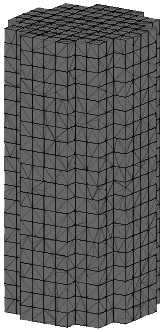
\includegraphics[width=4cm,height=7cm]{figures/Amir_ME5_Lattice_Setup.png}
\subcaption{}
\label{fig:Amir_ME5_Lattice_Setup}
\end{subfigure}
\begin{subfigure}[c]{0.5\textwidth}
\centering
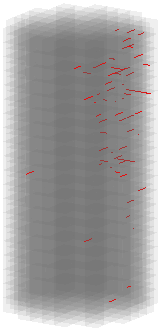
\includegraphics[width=4cm,height=7cm]{figures/Amir_ME5_Lattice_Frack.png}
\subcaption{}
\label{fig:Amir_ME5_Lattice_Frack}
\end{subfigure}
\caption{The (a) generated domain for simulation of the swelling processes, and (b) fracking paths shown with red surfaces}
\end{figure}

\begin{figure}[!ht]
\centering
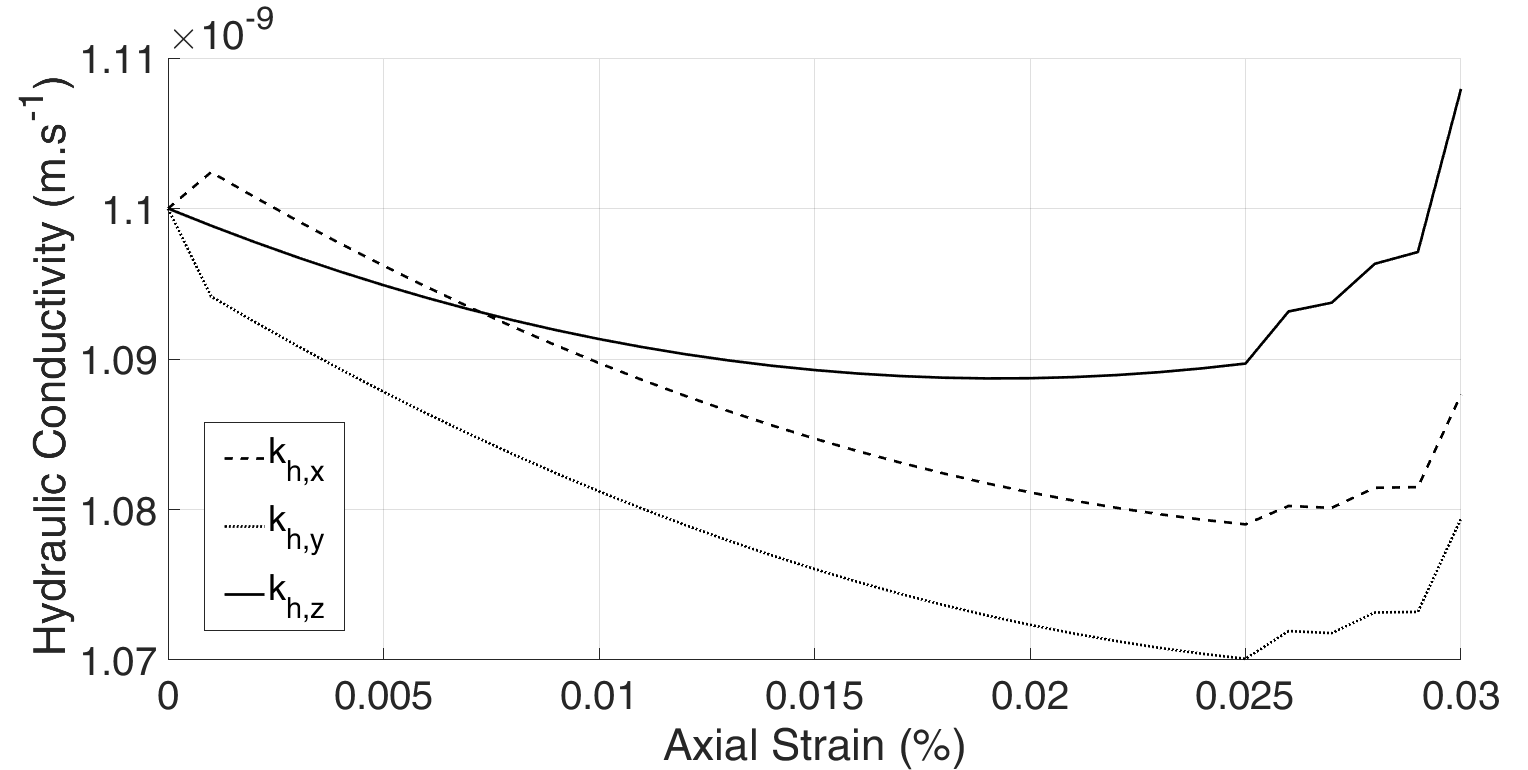
\includegraphics[width=8cm,height=5cm]{figures/Amir_ME5_Lattice_Drying.png}
\caption{The change of hydraulic conductivity along the axis for salt clay, swelling process}
\label{fig:Amir_ME5_Lattice_Drying}
\end{figure} 

%OK\todo[inline]{[UFZ] Keita will you contribute to this MEX?}
%OK\todo[inline]{I plan to contribute to the next one MEX 1.5}

%------------------------------------------------------------------------------
\subsection{Results and discussion}

The swelling of the salt clay under isostatic stress conditions of 4 bar, and a brine pressure of 1 bar is investigated. The flow rate, change of the samples volume as well as the permeability change during the swelling process is measured. The experimental results indicate the sudden increase in the flow volume after 8 days of the test procedure. Initially, the salt minerals re-crystallization may result in opening and closure of the pathways as indicated from experimental data. Eventually, the closure of the pathways in salt clay sample is observed, which resulted in decrease of the permeability. The lattice model using the elements swelling strain is implemented to simulate the change of the permeability during the test procedure. The integrated interface element method is used here to assess the change of the hydraulic aperture. The anisotropy of salt clay is neglected in this study. Therefore, the initial permeability and hydraulic aperture along different axis are assumed to be equal. The numerical result indicate the decrease of the hydraulic conductivity before the micro-fracking paths formation. The results do not correspond to the experimental data, as in the experimental data, increase of the permeability values were not observed. Further quantitative investigation of the results and validation of the lattice model is required. 